\documentclass[14Q,twocolumn]{jsarticle}
\usepackage[dvipdfmx]{graphicx}
\usepackage{wrapfig}
\usepackage{float}
\usepackage{otf}
\usepackage{longtable}
\usepackage{ulem}
\usepackage{ascmac}
\usepackage{multicol}
%%%%%
\makeatletter
\newenvironment{tablehere}
  {\def\@captype{table}}
  {}
\newenvironment{figurehere}
  {\def\@captype{figure}}
  {}
\makeatother
%%%%%%
\setlength{\textwidth}{160truemm}      % テキスト幅: 160mm
\setlength{\fullwidth}{\textwidth}     % ページ全体の幅
\setlength{\oddsidemargin}{0mm}   % 左余白
\setlength{\topmargin}{-10mm}       % 上余白
\setlength{\textheight}{240truemm}     % テキスト高さ: 297-(30+30)=237mm
\pagestyle{empty}
\title{GIS概論}% 文書のタイトル
\date{2018年9月18日}
\author{厚沢部町 石 井 淳 平}              % 著者

%------------------------------
\begin{document}
\maketitle
%\begin{multicols}{2}
\section{何を「GIS」と呼ぶのか}
「空間的な情報の取り扱いについて、コンピュータを用いてシステム化したもの」\footnote{
金田明大 2001「考古学研究とGIS」『考古学のためのGIS入門』古今書院,pp1-20
}
という説明が簡潔です。
「遺構配置図に遺物の出土地点をプロットして、等高線を上書きする」という作業をコンピュータ上で行えば、「GIS」といえます。これらの作業を手作業で行うことも可能ですが、「縄文中期前半の土器群だけを抽出する」という種類の作業を繰り返すうちに、人間には不可能な作業量に近づいていきます。また、「土器の出土量に対する石器の出土量の比率の空間分布」のように統計処理を含んだ処理を人間が正確に行うことは難しくなります。空間情報を含んだ複雑で膨大な処理を行うためのコンピュータソフトウェアが必要となります。

%%%%
\section{GISにできること}
空間情報のあるデータならどんなものでも対象になります。一般的には地理情報とはみなされない遺物の実測図や写真をGISソフトウェアで活用することも可能です。GISで行われているのは次のような作業です。

\begin{figurehere}
\centering
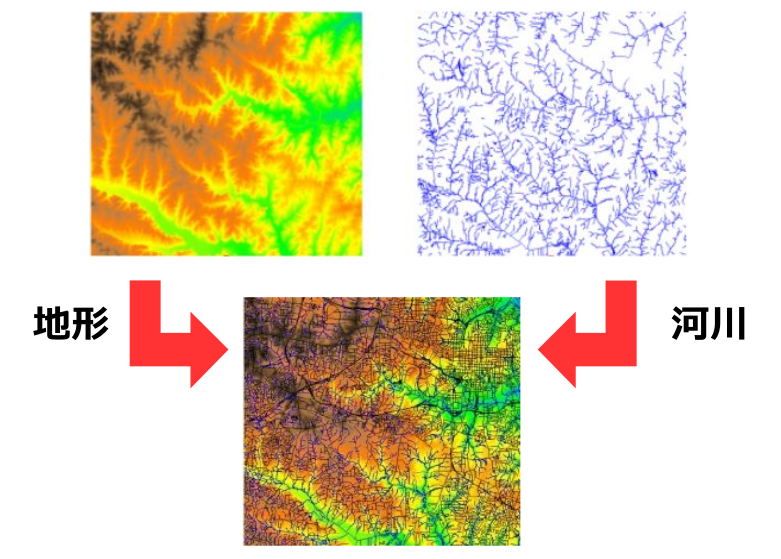
\includegraphics[width=1\linewidth]{exp01.png}
\caption{異なるデータの重ね合わせ(田中淳2018「QGIS初級編version3.03」,FOSS4G 2018 Hokkaido ハンズオン資料)}
\end{figurehere}

\begin{figurehere}
\centering
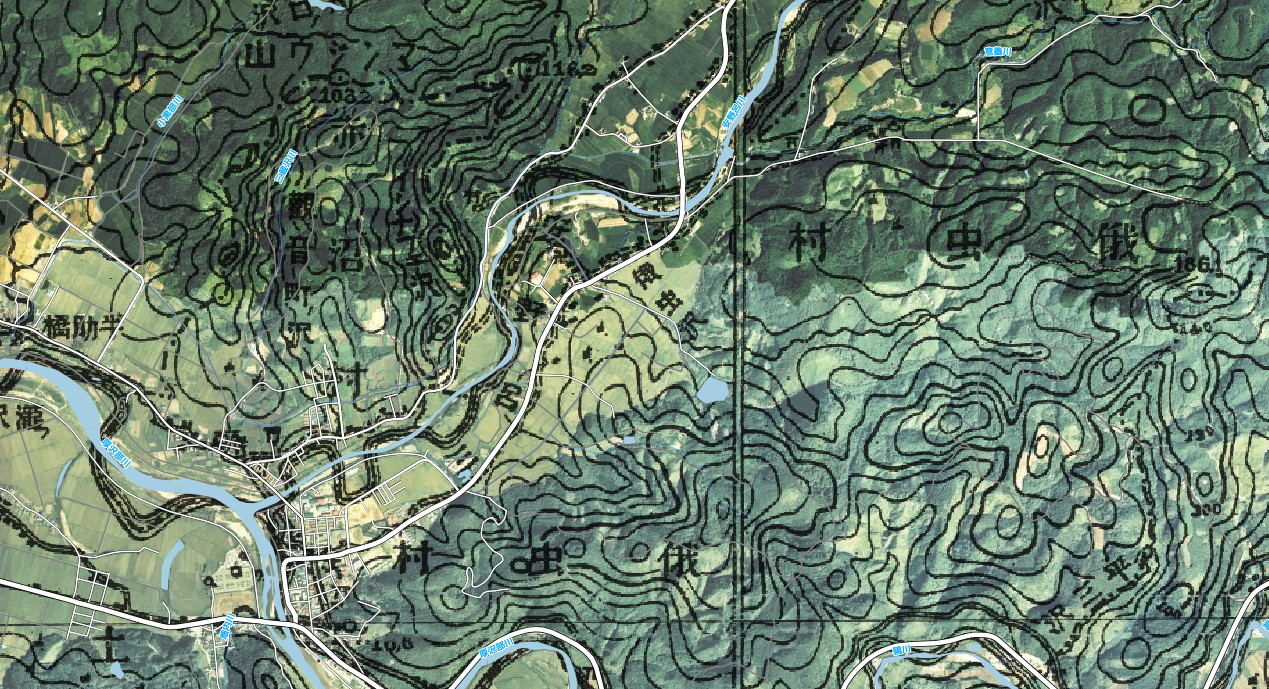
\includegraphics[width=1\linewidth]{exp04.png}
\caption{国土地理院旧版地形図と航空写真、現代の道路・河川の重ね合わせ}
\end{figurehere}

\begin{figurehere}
\centering
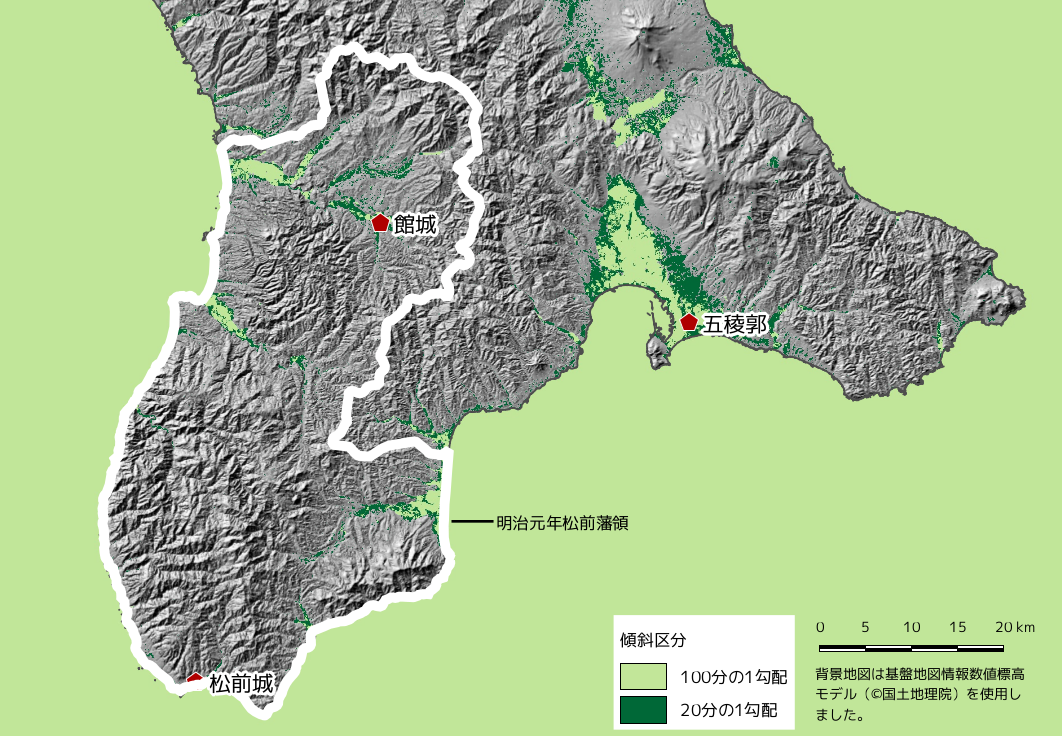
\includegraphics[width=1\linewidth]{exp05.png}
\caption{標高データから土地傾斜区分図を作成}
\end{figurehere}

\begin{figurehere}
\centering
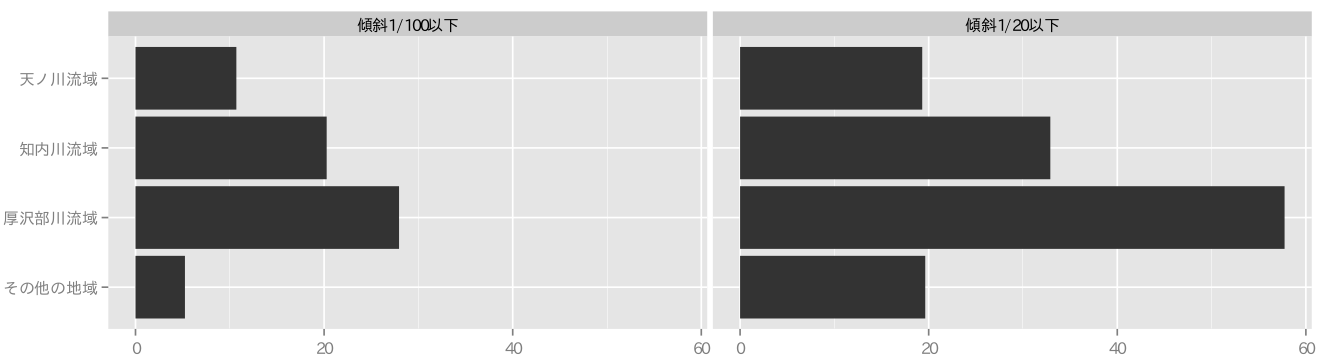
\includegraphics[width=1\linewidth]{exp06.png}
\caption{土地傾斜区分図からグラフを作成}
\end{figurehere}

\begin{itemize}
\item 最短経路・コスト距離
\item 傾斜算出、画像強調
\item 気象等観測データの補間
\item 属性に基づいたデータベース処理
\end{itemize}

%%%%
\section{ベクタデータ}
\subsection{ベクタデータの種類}
\begin{itemize}
\item ポイント=点データ
\item ライン =線データ
\item ポリゴン=面データ
\end{itemize}

\subsection{ベクタデータの形式}
「座標で地図を表現するデータ」をベクタデータと呼びます。データの種類には次のようなものがあります。

\subparagraph{Shapefile}
ESRI社のフォーマット。デファクトスタンダード。データベースとしては古い構造(.dbf)を維持しているため最新のデータベースでできることができない場合があります。GISでのトラブルの多くがシェープファイルに由来している側面があります。
\subparagraph{Spatialite}
データベースエンジンにSQliteを使用。シンプル・軽量・高機能。ポストシェープファイル。
\subparagraph{GPX}
GPSで使われるファイル形式。GISにインポートした後は別のファイルに変換することが一般的です。
\subparagraph{CSV}
カンマ区切りテキスト。x座標とy座標があればGISデータとして使えます。表計算ソフトで扱えてシンプル極まりない構造ですが、ポイントデータしか表現できません。
\subparagraph{GeoJson}
Javascriptをベースにつくられたデータ格納形式。JSONのGIS版。

これまではShape形式がスタンダードでしたが、ウェブ系のエンジニアやデータベースの専門家が地理情報システムを扱うことが増えたため、様々な形式のデータが登場しています。「とりあえずShape形式にしておけば大丈夫」という時代ではなくなってきたようです。



\begin{figurehere}
\centering
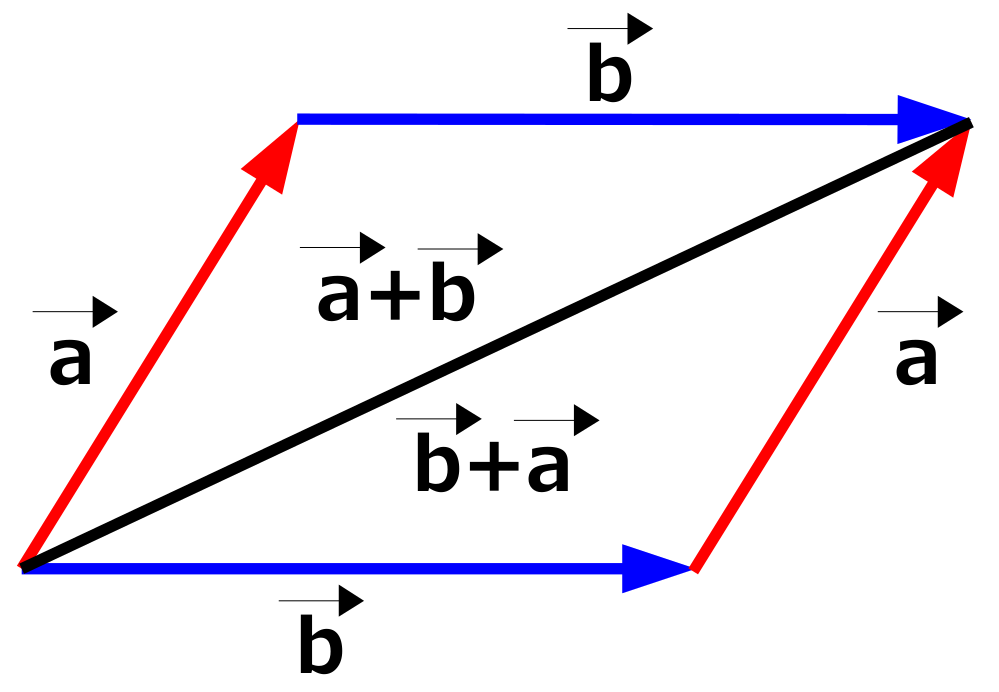
\includegraphics[width=1\linewidth]{vector01.png}
\caption{ベクタ画像の概念(田中淳2018)}
\end{figurehere}

%%%%
\subsection{ベクタデータの特徴}
ベクタデータの特徴は、地理情報をデータベースとして扱うことができる点です。データベースであるため次のような作業が可能になります。

\begin{itemize}
\item 出土層位ごとに遺物の分布図を作成する。
\item 包含層出土遺物のうち、竪穴の2m圏内から出土した遺物を抽出する。
\item 時代ごとに遺構図を表示する。
\end{itemize}

\begin{figurehere}
\centering
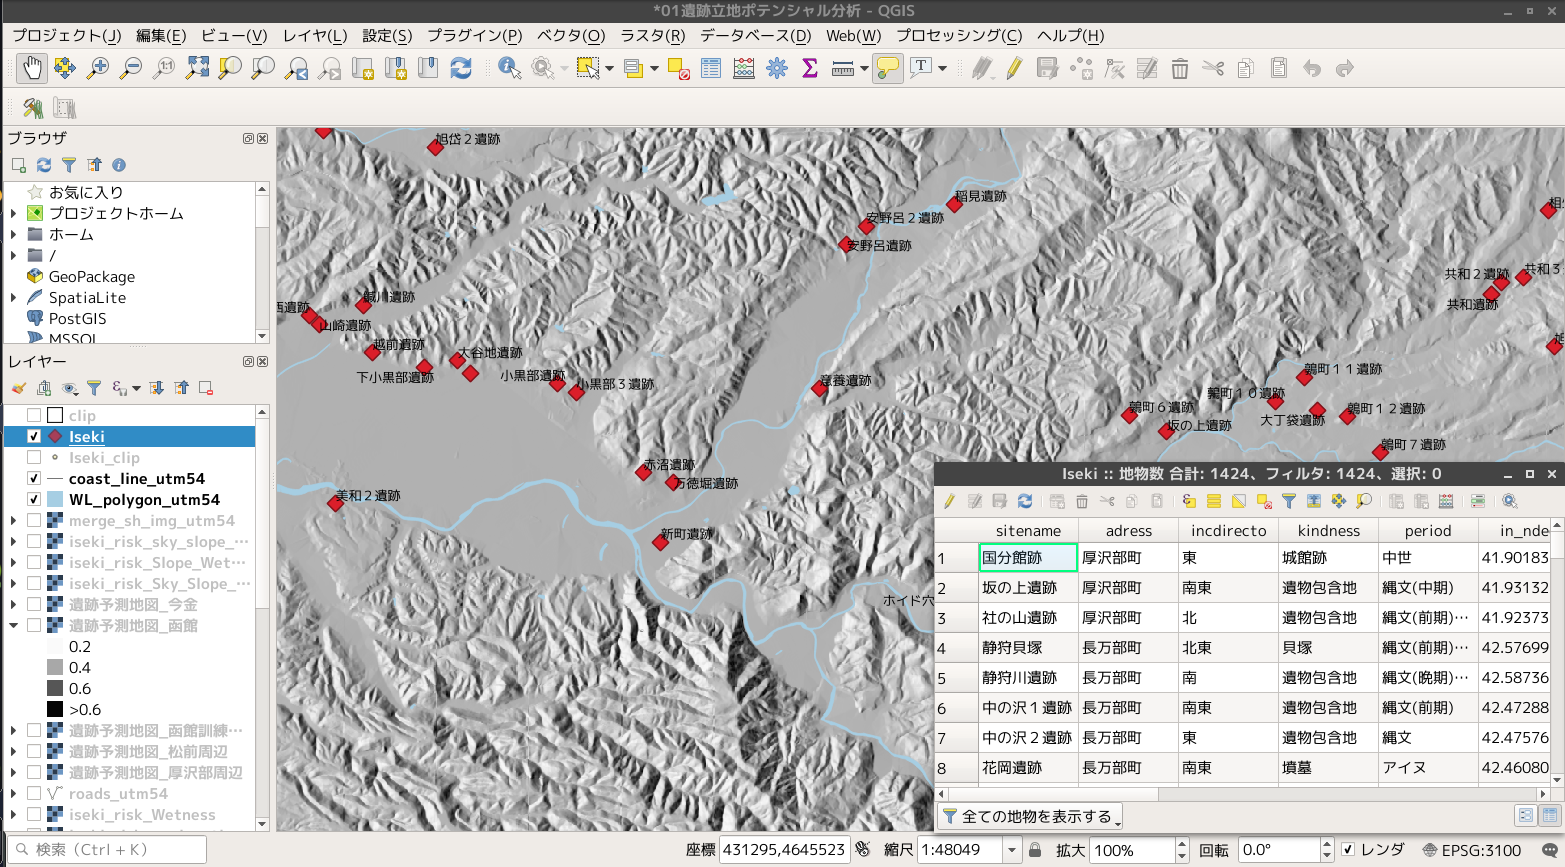
\includegraphics[width=1\linewidth]{vector02.png}
\caption{データベースとしてのベクタデータ}
\end{figurehere}

%%%%%
\section{ラスタデータ}
\subsection{ラスタデータの形式}
GeoTIFF一択です。GeoTIFFはオープンな規格で設計されており、当面ラスタデータはGeoTIFFが使用されるものと思われます。

%%%%
\subsection{ラスタデータの特徴}
航空写真や遺物実測図のように「絵的」なものと、標高データのような数値行列を「絵的」に表現したものにわけられます。標高データでは標高値をグレースケールの256階調に割り振ったり、任意のカラースケールに変換して表現します。GISの機能の一つとして、様々なラスタデータを透過的に重ね合わせて表現することが可能です。傾斜区分図や陰影図、曲率図などと組み合わせて「赤色立体図」や「CS立地図」などの新しい視覚表現も生み出されています。

\begin{figurehere}
\centering
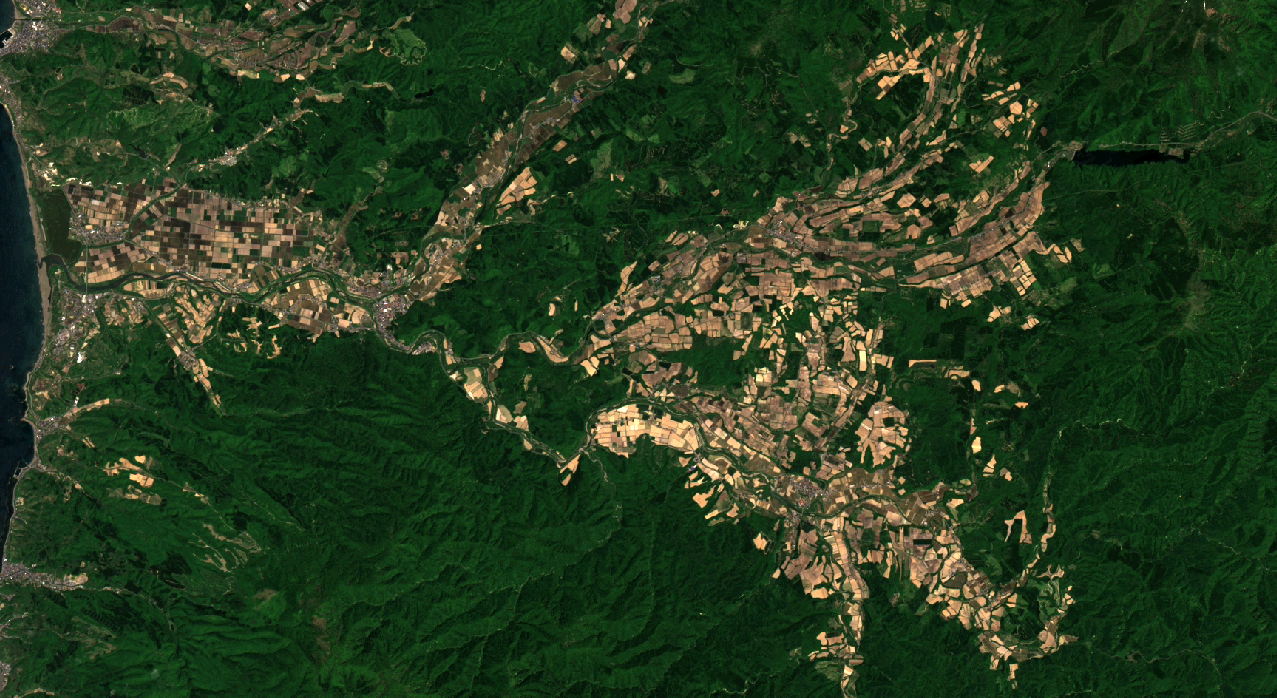
\includegraphics[width=1\linewidth]{rastar03.png}
\caption{絵的なラスタデータ(Landsat7衛星画像)}
\end{figurehere}

\begin{figurehere}
\centering
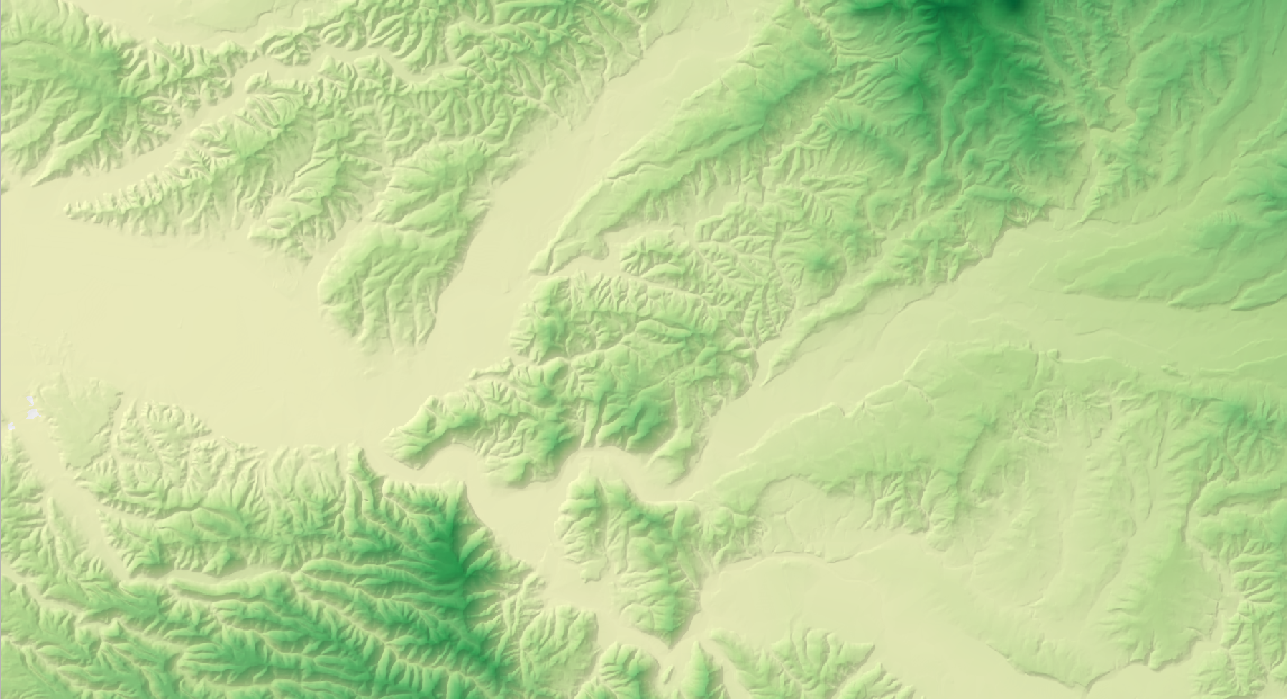
\includegraphics[width=1\linewidth]{rastar02.png}
\caption{データ行列のラスタデータ(数値標高モデル)}
\end{figurehere}

\begin{figurehere}
\centering
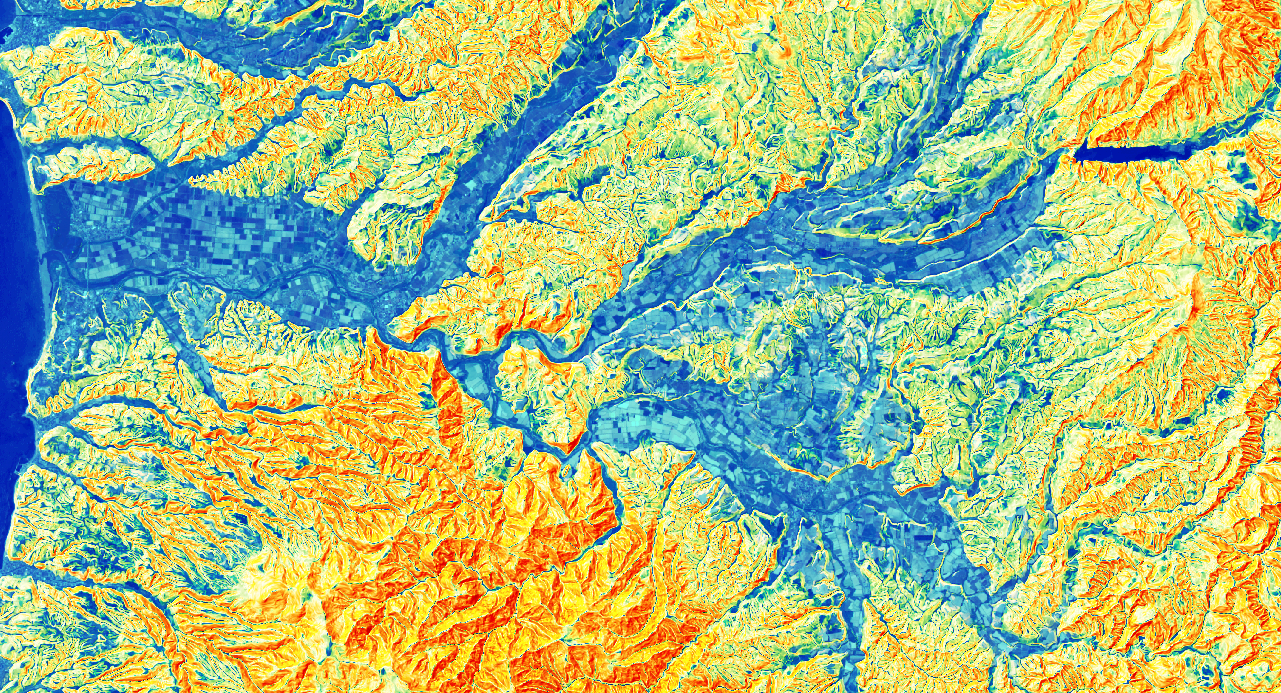
\includegraphics[width=1\linewidth]{rastar04.png}
\caption{衛星画像+傾斜区分図+陰影図}
\end{figurehere}

\begin{figurehere}
\centering
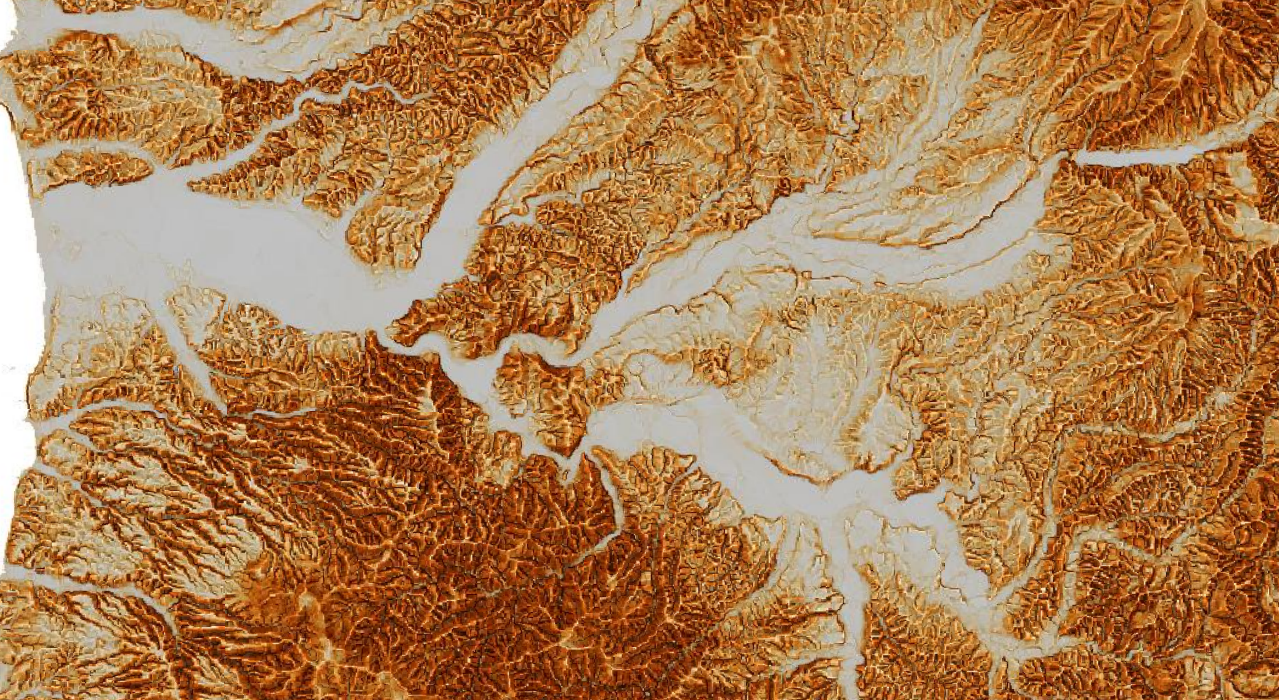
\includegraphics[width=1\linewidth]{rastar05.png}
\caption{微地形の判読に特化したCS立体図(北海道CS立体図)}
\end{figurehere}

%%%%
\section{測地系と座標系}
\subsection{測地系・座標系とは何か}
\begin{itemize}
\item 測地系=地球の形
\item 座標系=投影法とほぼ同義。球体の平面展開方法
\end{itemize}

\begin{figurehere}
\centering
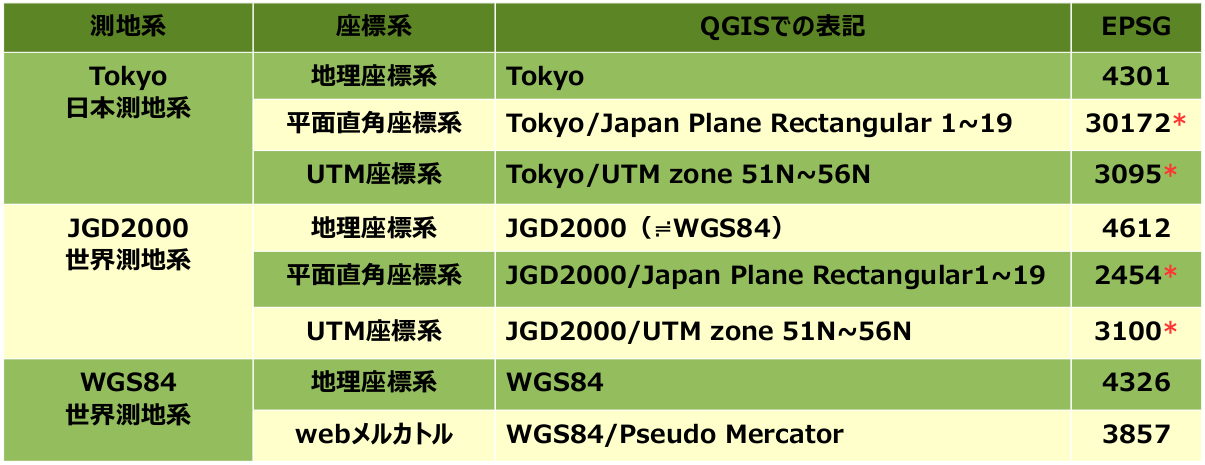
\includegraphics[width=1\linewidth]{sokuti01.png}
\caption{測地系と座標系一覧(田中淳2018)}
\end{figurehere}

%%%%
\subsection{測地系は何を選ぶべきか}
「世界測地系」\footnote{
世界測地系はGSR80という基準楕円体を採用した測地系。2002年施行の改正測量法により基本測量や公共測量は世界測地系に基づき測量を実施することが義務付けられました。いわゆる「新座標」です。それ以前の座標系は「日本測地系」です。
}
以外の選択肢はありません。現在公共事業や公費負担の事業として行われる発掘調査\footnote{
『公共測量の手引』(国土地理院企画部測量指導課2008,https://psgsv2.gsi.go.jp/koukyou/public/tebiki/tebiki.pdf)では文化財調査にともなう「現況把握のための空中写真撮影、レーザ測量、現況図作成など」は公共測量に該当するとされています。
}
で世界測地系以外の測地系を採用することは「違法」です。

\subparagraph{測量法第1条}
この法律は、国若しくは公共団体が費用の全部若しくは一部を負担し、若しくは補助して実施する土地の測量又はこれらの測量の結果を利用する土地の測量について、その実施の基準及び実施に必要な権能を定め(後略)

\subparagraph{測量法第11条第1項}
基本測量及び公共測量は、次に掲げる測量の基準に従つて行わなければならない。\\
一 位置は、地理学的経緯度及び平均海面からの高さで表示する。ただし、場合により、直角座標及び平均海面からの高さ、極座標及び平均海面からの高さ又は地心直交座標で表示することができる。

\subparagraph{測量法第11条第2項}
前項第一号の地理学的経緯度は、世界測地系に従つて測定しなければならない。

%%%%
\subsection{座標系は何を選ぶべきか}
GISで運用する上で3つ選択肢が考えられますが、地方自治体等での運用実績を勘案すると平面直角座標系を選ぶことが適切と考えられます。

\subparagraph{緯度経度系}
座標としては馴染み深いものですが、GISで扱う上では空間演算処理ができず不適切です。また、自治体の他の測量成果との整合をとることも難しくなります。

\subparagraph{UTM座標系}
赤道を原点とする投影座標系です。比較的広範囲を扱うことに優れているといわれます。自治体ではあまり一般的ではありません。

\subparagraph{平面直角座標系}
自治体で一般的に利用されている座標系です。特に理由がなければ平面直角座標系を選択することが無難です。

\begin{figurehere}
\centering
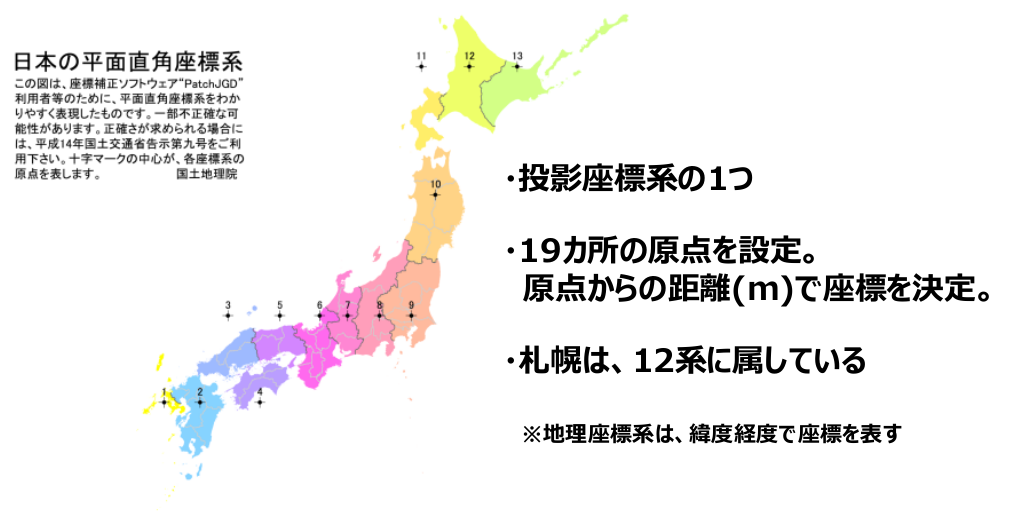
\includegraphics[width=1\linewidth]{zahyou01.png}
\caption{平面直角座標系(田中淳2018)}
\end{figurehere}

%%%%
\section{緯度経度系をどうするか}
測量法上は測量成果は原則として緯度経度系を使用することとなっています。平面直角座標系等は「場合によ」って使用可能というのが法的な位置づけです。発掘調査報告書抄録の遺跡位置は『行政目的で行う埋蔵文化財の調査についての標準(報告)』(文化庁埋蔵文化財発掘調査体制等の整備充実に関する調査研究委員会2004)に基づいて「遺跡のほぼ中心と思われる位置を度分秒の単位で記入する。国土地理院2万5千分の1地形図等を利用して算出する」こととされています。

緯度経度系の使用はGISでは推奨されませんが、抄録用位置情報は度分秒形式の緯度経度で表示する必要があります。「遺跡の位置」に厳密性を求めていくと「遺跡とは何か」という途方もない課題にたどりつきますので、本研修では触れませんが、代表点の求め方は次の3つが考えられます。

\begin{itemize}
\item 遺跡の範囲が確定している場合には遺跡範囲の幾何学的な重心点
\item 遺跡の地番が確定している場合は所在地番の幾何学的な重心点
\item 遺跡範囲が確定していない場合は25000分1地形図上で目視によりもっとも中心らしいと思われる点とする
\end{itemize}

幾何学的な重心点の算出はGISソフトウェアで行います。目視による方法では地理院地図による座標の取得が簡単です。

\begin{figurehere}
\centering
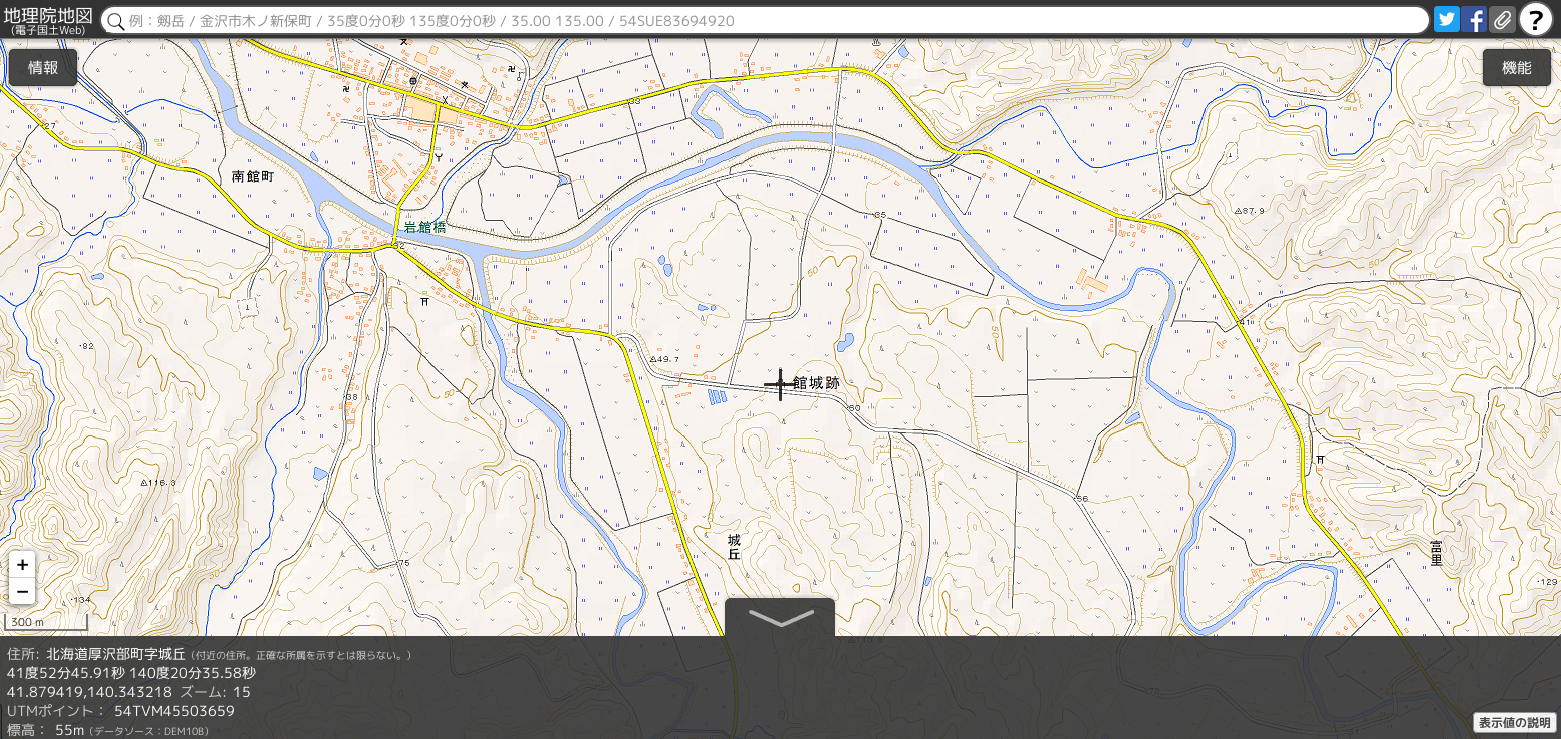
\includegraphics[width=1\linewidth]{shouroku01.png}
\caption{地理院地図による緯度経度の取得}
\end{figurehere}

%\end{multicols}
\end{document}
